\chapter{Theory}
I will attempt to explain all theory required to understand this project using a top-down approach. By first explaining the big picture in which this research project is located we hope to avoid the reader getting lost in the details and misunderstanding the purpose of this report. 

\section{Force estimation}
When moving a limb the most intuitive way of describing it is a change in position, moving your hand from A to B. However, a more objective way of describing this movement is in terms of forces applied on a mass:
\begin{itemize}
    \item Muscles contract
    \item This causes a force to be applied on a mass, or a torque around a pivot point
    \item This force results in an acceleration in a certain direction
    \item This acceleration is maintained for a certain period of time
    \item The entire process is repeated for deceleration using visual feedback for fine tuning of forces
    \item Your limb has arrived at a new location.
\end{itemize}

Understanding this reasoning of moving a limb in terms of forces being applied by contracting muscles is vital because it forms the basis for recognizing a user's intent. EMG can be used to measure the degree of contraction of a muscle, and by measuring the degree of contraction of two antagonistic muscles it is possible to calculate how much force is applied in a certain direction which signals a desire for this limb to move. Even if the limb is not present and replaced by a prosthesis this idea of forces moving a mass will still apply, and thus EMG can be used as a human-machine interface.

So to summarize the basic concept of force estimation:
\begin{itemize}
    \item Movement of a limb is the result of a force acting on that limb
    \item This force is the result of certain muscles contracting stronger than other muscles
    \item The contraction of these muscles can be measured using EMG
    \item EMG can be used to estimate limb movement
\end{itemize}

\section{sEMG signal properties}

\begin{figure}[h!t]
	\begin{center}
		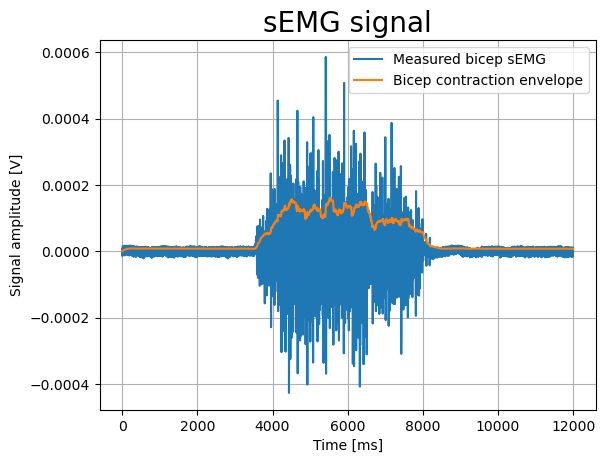
\includegraphics[width=1.0\columnwidth]{images/sEMG_signal_example.png}
	\end{center}
	\caption{sEMG signal measured from bicep during contraction}
	\label{fig:sEMG_signal_example}
\end{figure}

\begin{figure}[h!t]
	\begin{center}
		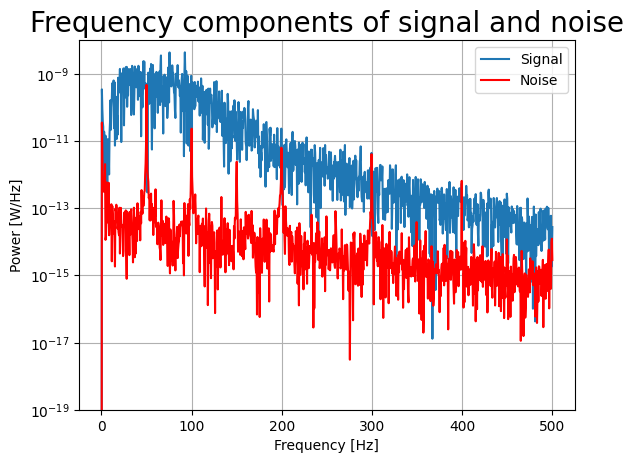
\includegraphics[width=1.0\columnwidth]{images/sEMG_fft_signalnoise_example.png}
	\end{center}
	\caption{Frequency components of signal and noise in an sEMG signal. 
    Noise is taken to be 0-2s and Signal is taken to be 5-7s in \ref{fig:sEMG_signal_example}}
	\label{fig:sEMG_fft_signalnoise_example}
\end{figure}

\begin{figure}[h!t]
	\begin{center}
		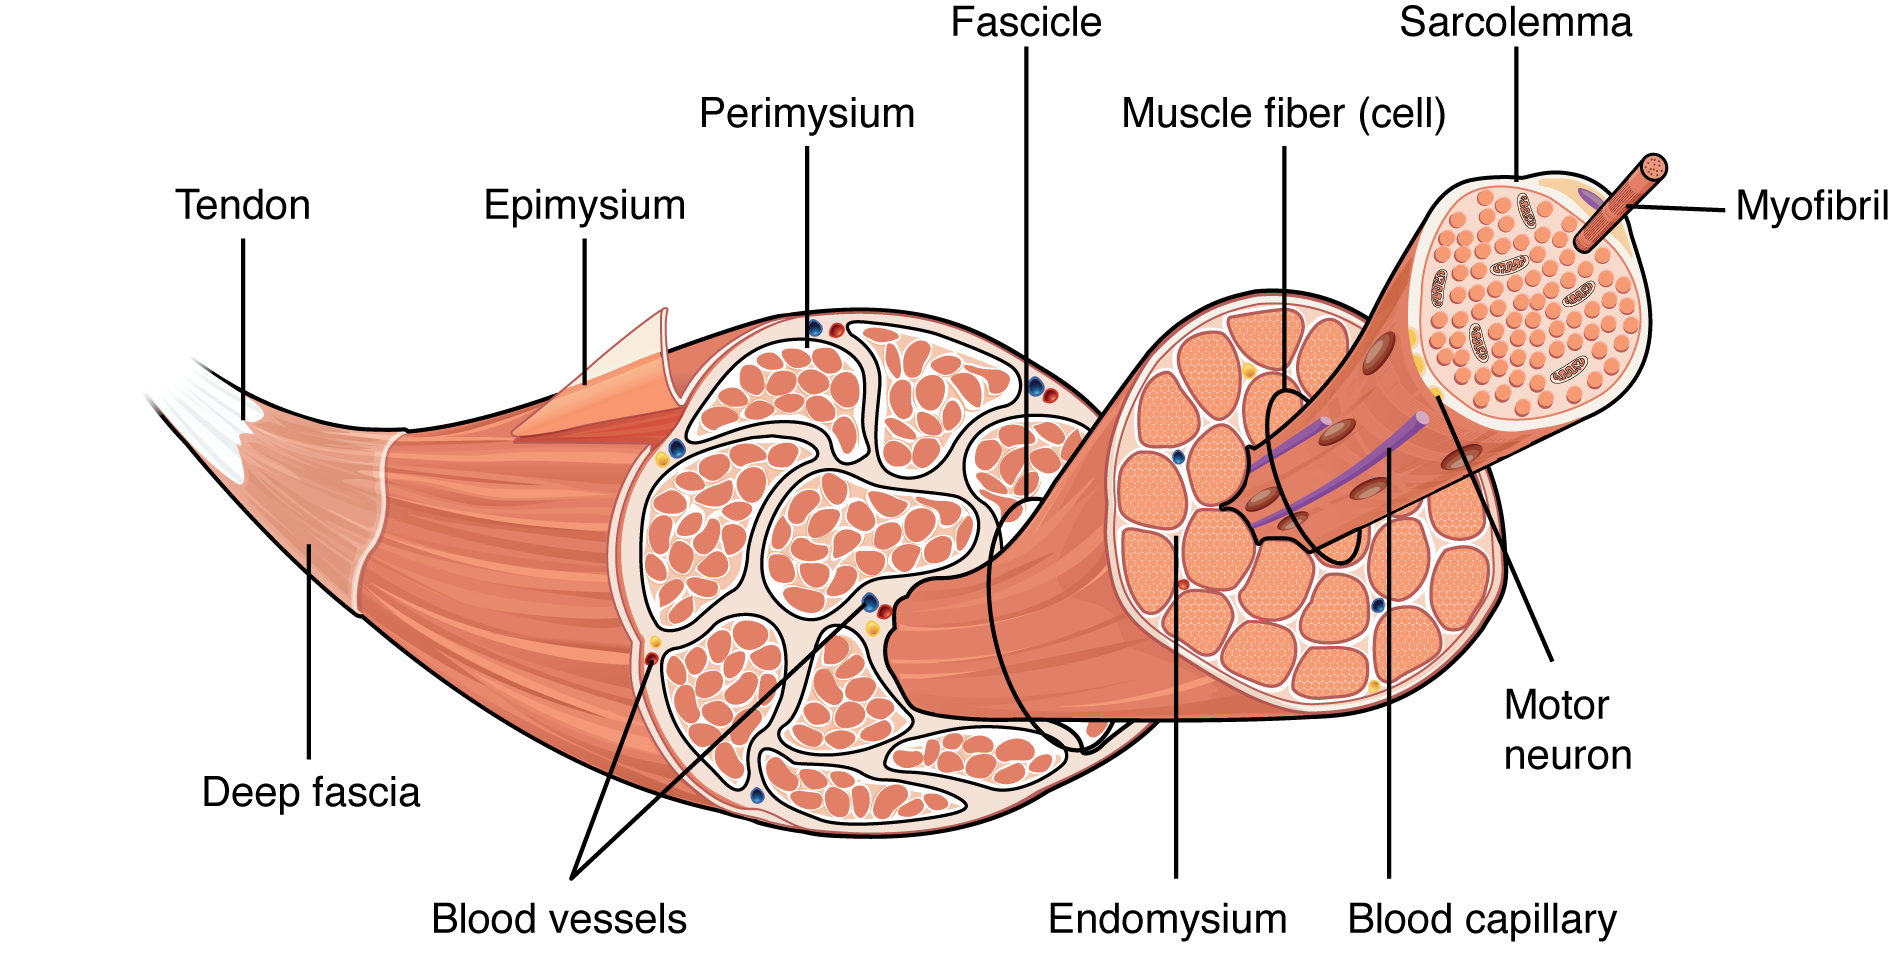
\includegraphics[width=1.0\columnwidth]{images/muscle_anatomy.png}
	\end{center}
	\caption{Anatomy of a muscle \cite{muscle_anatomy}}
	\label{fig:muscle_anatomy}
\end{figure}

\textcolor{red}{Todo: Find source that further explains muscles and EMG signals to refer to for further reading}

Figure \ref{fig:muscle_anatomy} illustrates the anatomy of a muscle which may be useful in this section. 
A large skeletal muscle such as the bicep consists of hundreds of thousands of small muscle fibers. These muscle fibers are divided into groups called motor units, and each motor unit is connected to a motor neuron which is a special type of very long brain cell that runs through the spinal cord. A contraction of a skeletal muscle is the result of many muscle fibers contracting individually and repeatedly. The contraction of these muscle fibers is the result of an action potential caused by the motor neuron, and this action potential is a measurable (but very small) voltage. When measuring the surface EMG of a contracting skeletal muscle the result is the aggregate of the small voltages from all contracting muscle fibers. This manifests itself into a signal resembling white noise where the amplitude of the noise correlates to the number of contracting muscle fibers and thus to the amount of contraction the skeletal muscle experiences. This is shown in \ref{fig:sEMG_signal_example} where a maximum voluntary contraction (MVC) is measured from a bicep.
 
So to summarize: to determine the degree of contraction of a skeletal muscle we simply need to determine the amplitude of the noise at the surface of the muscle.

From this point onwards I will refer to the 'noise' generated by muscle contraction as 'the signal'. This is done because noise is usually unwanted, but the signal caused by muscle contraction is the opposite of unwanted: It precisely what we're trying to measure! 

Unfortunately, when measuring sEMG signals it is impossible to measure solely the signal generated by muscle contraction. The signal may be polluted by other signals coming from the surrounding environment (such a 50 Hz power lines nearby) or from the amplifier used to amplify the measured signal. So in reality we are measuring a combination of our desired signal from muscle contraction, and the undesired noise from the environment and amplifier. An illustration of the frequency content of the signal and noise is shown in figure \ref{fig:sEMG_fft_signalnoise_example}. Note how the the noise has large peaks at 50Hz and multiples of 50Hz; This is the noise generated by the power lines. 

The ratio between how much of the measured signal is actual desired signal and how much is undesired noise is called the Signal to Noise Ratio (SNR) and is defined as the signal power divided by the noise power \textcolor{red}{(SOURCE) (EQUATION)}. As the amount of desired signal increases and the amount of noise decreases, the accuracy with which the force can be estimated from the contraction also increases. In other words, a larger SNR results in a more accurate estimation. We can increase the SNR by removing noise, and for this exact purpose 'filters' were invented.

\section{Filters}
% Introduce basic concept of filters
At a fundamental level filters are simply a tool to remove something unwanted (noise) that is mixed with something wanted (signal). In signal processing filtering is achieved by decomposing a measured signal into repeating patterns and subsequently deciding which patterns should be included and which patterns should be removed. Figure \ref{fig:filter_example} displays how a time-domain signal can be represented in the frequency domain to display informationa bout which frequencies are present in the signal.

\begin{figure}[h!t]
	\begin{center}
		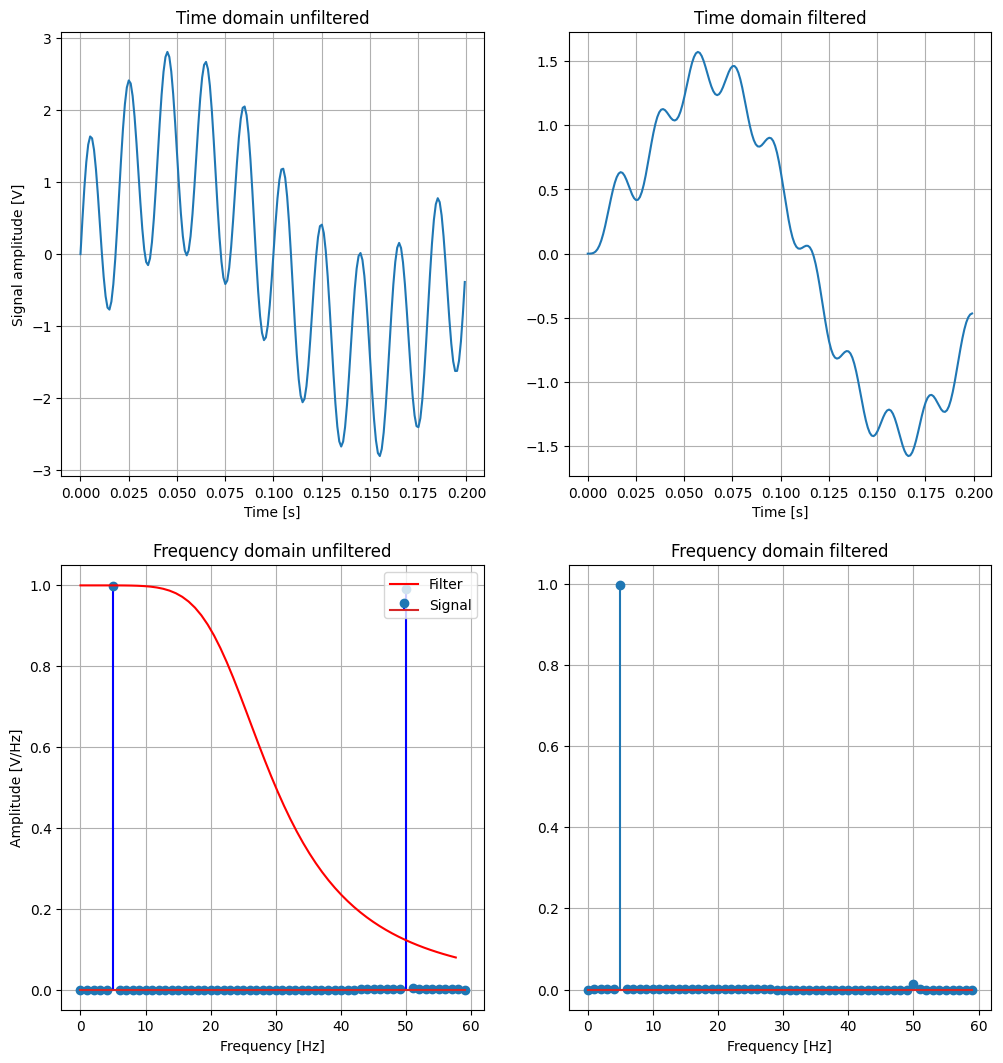
\includegraphics[width=1.0\columnwidth]{images/filter_example.png}
	\end{center}
	\caption{Filtering a signal. In the top-left figure there is a low-frequency signal polluted by a 50Hz signal. The frequency plot in the bottom-left shows these frequencies. By applying the low-pass filter as displayed in the bottom-left it is possible to filter out the higher 50Hz frequency. The resulting filtered signal can be seen in the top-right, showing that there is still a little bit of noise left. This is also visible in the bottom right showing the frequency contents of the signal after filtering}
	\label{fig:filter_example}
\end{figure}

% Explain difference between analog digital and continuous and discrete
The physical world is inherently analog. Any property that changes from one value to another (such as a change in as wind speed, water level, voltage or age) will at some point have been equal to any value between the start and end value; Between 1 and 2 Volt there are infinite values with infinite decimals \textcolor{red}{(SOURCE)}. Computers sadly don't have infinite memory to store all these values and therefore to measure a continuous signal it needs to be sampled at equidistant points in time. This turns an analog continuous signal into a digital discrete signal. Even though filtering is possible in the analog domain, it is much less complicated and more flexible to filter in the digital domain \textcolor{red}{(NEED CITATION)}.

\textcolor{red}{< Image of analog vs digital as illustration of above text >}

In the digital domain the basic concept of a filter is as simple as it is magical. A filter (usually) consists simply of a set of values called the filter coefficients. The input (measurements) is multiplied with the filter coefficients to create the output. That is, the latest measurement is multiplied with the first filter coefficient, the previous measurement is multiplied with the second filter coefficient, and so on. This can also be interpreted as multiplying each filter coefficients with a delays input sample. Figure \ref{fig:wiki_digital_filter_working} shows the working and standard notation of a digital filter.
By carefully choosing the number and value of filter coefficients it is possible to attenuate specific frequencies while not influencing other frequencies such as the effect shown in \ref{fig:filter_example}.

\begin{figure}[h!t]
	\begin{center}
		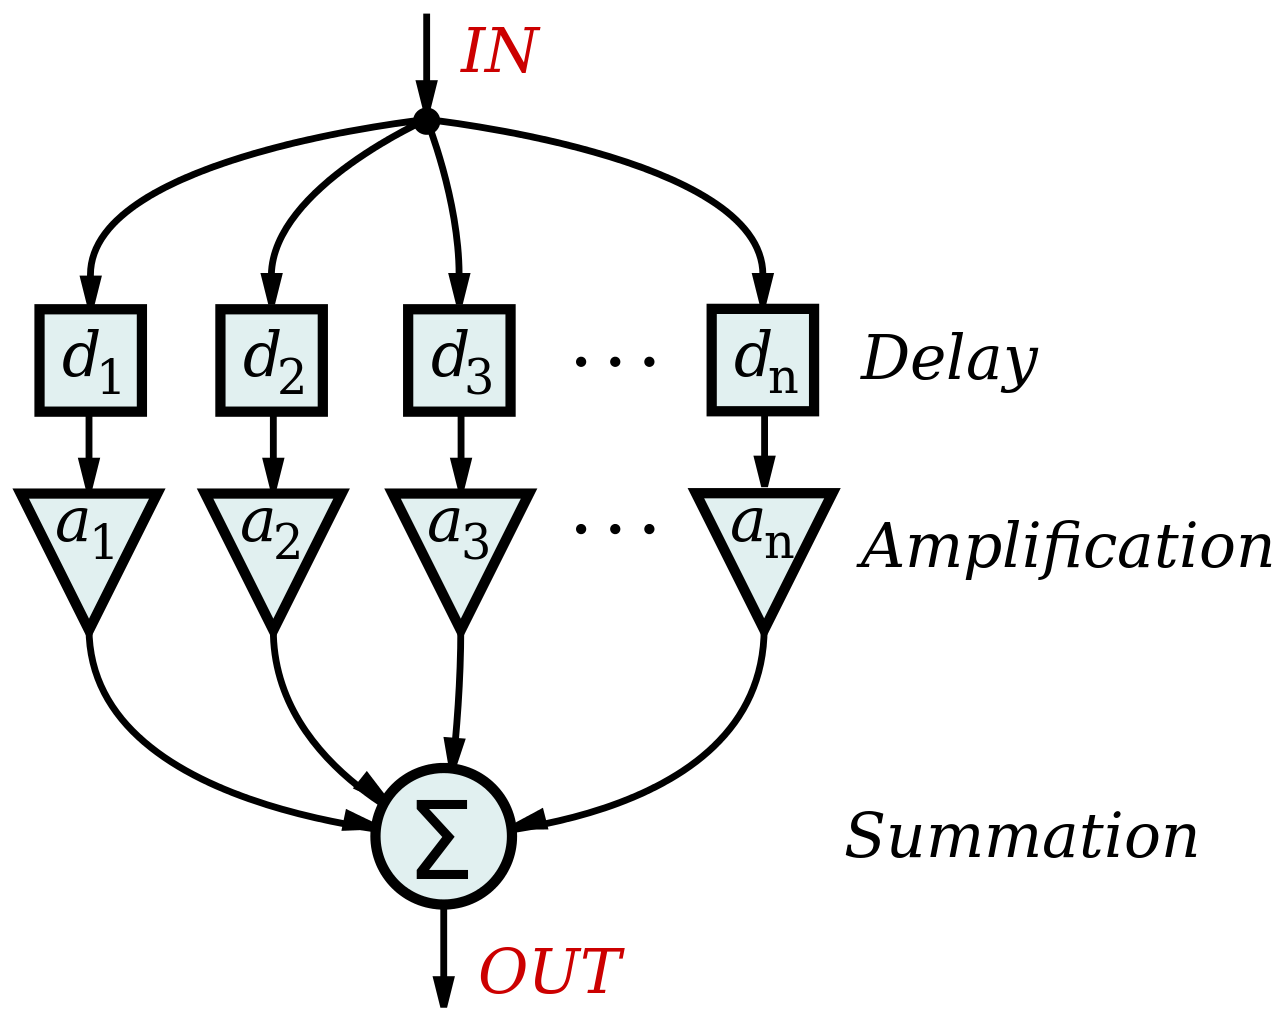
\includegraphics[width=1.0\columnwidth]{images/wikipedia_fir_digital_filter.png}
	\end{center}
	\caption{The functioning of a digital filter. The filter coefficient at index $i$ is multiplied by the input that is delayed $i$ samples \cite{wikipedia:digital_fir_filter_image}}
	\label{fig:wiki_digital_filter_working}
\end{figure}

\subsection{Static filters, Wiener filter, Adaptive filters}
If a filter is static (e.g. high-pass, low-pass, band-pass, or band-stop) it simply means that the amount of filter coefficients and the values of the filter coefficients are predetermined. These filters are very popular due to their simplicity in terms of finding the value of the filter coefficients. If a signal is expected to be between 90 and 100 Hz, a bandpass filter can be created even before the signal is measured that removes all signal components \textit{except} those between 90 and 100 Hz just by multiplying some values together. 

\begin{figure}[h!t]
	\begin{center}
		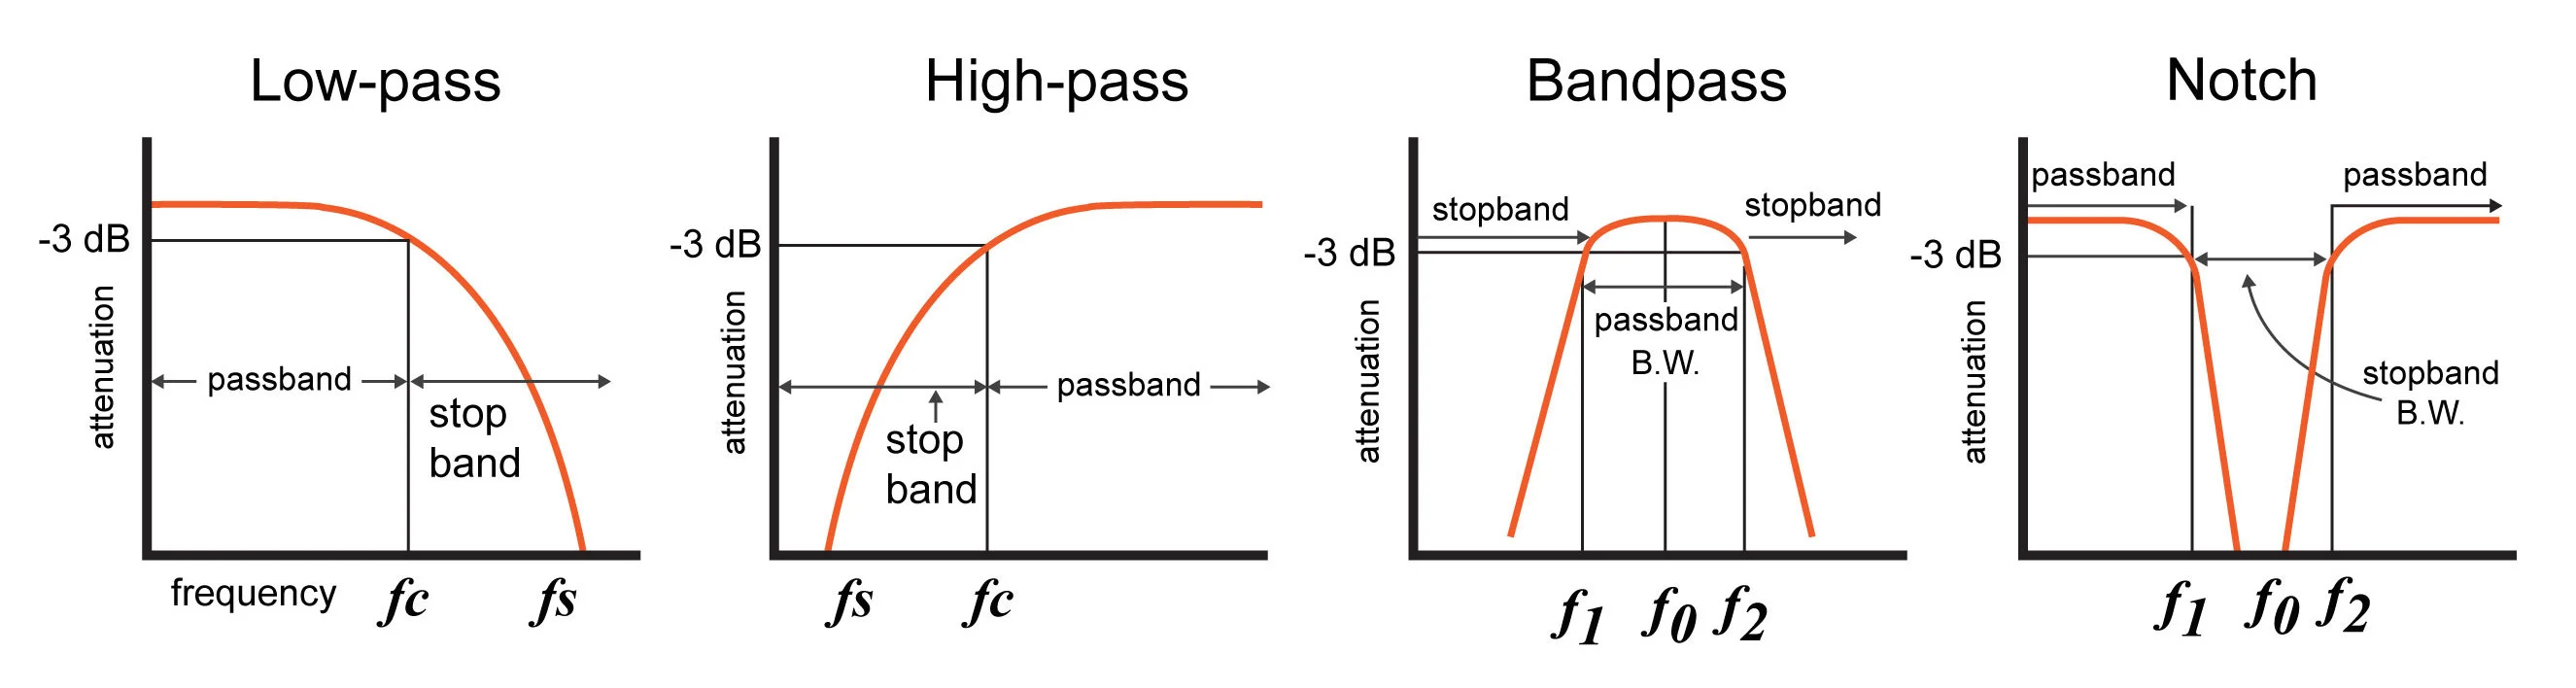
\includegraphics[width=1.0\columnwidth]{images/Davis_intro_to_filters_filter_types.png}
	\end{center}
	\caption{Frequency responses of the common 4 static filters \cite{intro_to_static_filters}}
	\label{fig:static_filters}
\end{figure}

A Wiener filter is a static filter that removes the frequency contents of noise from the frequency contents of a signal. In other words, the Wiener filter attenuates the frequencies that are present in noise so that when the filter is applied to a signal that is polluted by noise with the same frequency contents it effectively removes the noise. This is done by measuring two things: The signal that is corrupted by noise, and the noise separately. For example when measuring an sEMG signal an additional channel is used to measure the signal of a non-contracting muscle to gather only the present noise.
The Wiener filter requires both the signal and the noise to be stationary, i.e. the spectral density does not change over time, and results in a linear time-invariant filter \cite{wiki:Stationary_process} \cite{difference_stationary_nonstationary}. An example of the Wiener filter frequency response can be found in figure \ref{fig:wiener_filter_response}.

\begin{figure}[h!t]
	\begin{center}
		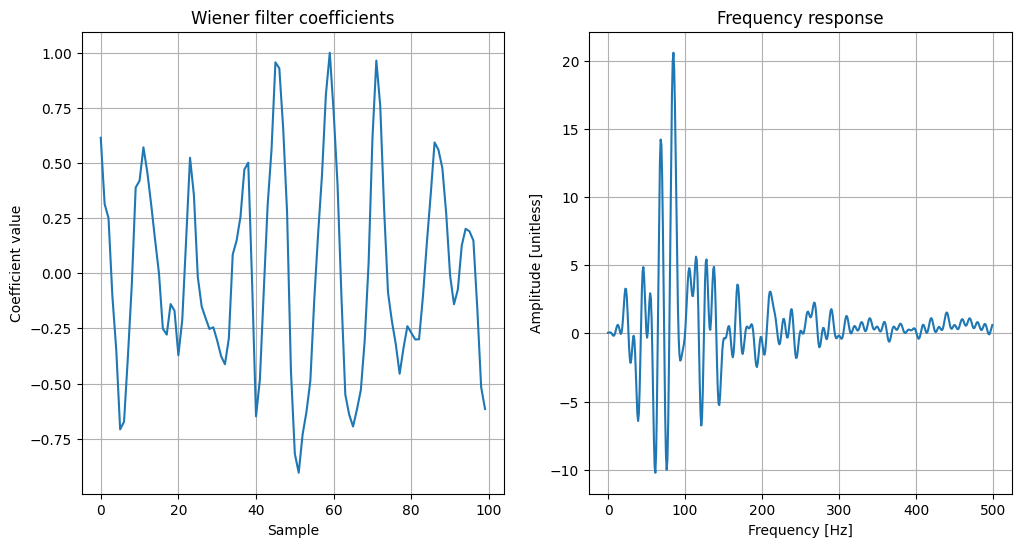
\includegraphics[width=1.0\columnwidth]{images/wiener_filter_response.png}
	\end{center}
	\caption{Sample values and frequency responses of a Wiener filter}
	\label{fig:wiener_filter_response}
\end{figure}

Adaptive filters expand on the idea of using knowledge of the spectral domain to create a filter by only using a subset of the input data (last $n$ samples). By re-calculating the filter coefficients with new data it is possible to update the filter to match a changing spectral density. 

Adaptive filters are applied in the same way as static filters by just multiplying the filter with measurements. However, the  method of finding the filter coefficients is different. Instead of deciding beforehand what frequencies you want to have removed, you measure the noise and determine its frequency spectrum. Then you tune the filter coefficients to remove these frequencies from the measurements (which also includes noise) leaving only the desired signal. This filter is used in environments where the noise frequency spectrum is not known beforehand, or when the frequency behaviour of the noise may change over time. Common applications of adaptive filters include speech recognition and noise-cancelling headphones! \cite{wiener_vs_adaptive_realtime_noisecancellation}

\textcolor{red}{(TODO: MATHEMATICAL DEFINITION OF FINDING COEFFICIENTS IN ADAPTIVE FILTERS) }

\textcolor{blue}{
=> LMS algorhitm
=> """"Instead of computing as suggested by
Wiener-Hopf equation, in LMS the coefficients are adjusted
from sample to sample in such a way as to minimize the MSE.... The LMS algorithm is based on steepest descent algorithm. ... """" => Wiener-hopf algorithm calculates $W_{opt}$ (Performance of Wiener Filter and Adaptive Filter for Noise Cancellation in Real-Time Environment, paper).}

\textcolor{red}{< IMAGE OF ADAPTIVE FILTER DIAGRAM >}

\subsection{FIR vs IIR}
Another subdivision within filter design is concerned with the type of possible responses to a specific input (impulse) and whether or not this can go to infinity.

The previously discussed filters were all described as Finite Impulse Response (FIR) filters. This means that the output is the result of multiplying the filter coefficients with the input. This type of filter is always stable and the output can never go to infinity as long as the input does not go to infinity.

An Infinite Impulse Response filter calculates the output using two sets of filter coefficients. The first set of filter coefficients is used to multiply with the input just like a FIR filter, but the second set of filter coefficients is used to multiply with previous \textit{outputs}. This means that there is now a feedback loop in the system, and a system with feedback can become unstable. Unstable in this case means that there is a possibility of positive feedback loop where increasing output values result in future output values also increasing, eventually going to infinity. Even though this feedback and possible instability may sound like a downside, it also results in shorter filter length and thus fewer computations required per filter operation. This could especially provide beneficial in low memory and low compute power environments like in prostheses \cite{fir_vs_iir}.

Both static and adaptive filters can be implemented as both FIR or IIR filters. An adaptive IIR filter offers the potential to meet desired performance levels with much less computational complexity. However, the possibility for the system to become unstable combined with the fact that filter coefficients are adjusted automatically leads to a high-risk high-reward scenario due to a loss of control and hard to predict behaviour. Background material on adaptive IIR materials can be found in chapter 23 of the Signal Processing Handbook \cite{digital_signal_processing_handbook}.

\begin{figure}[h!t]
	\begin{center}
		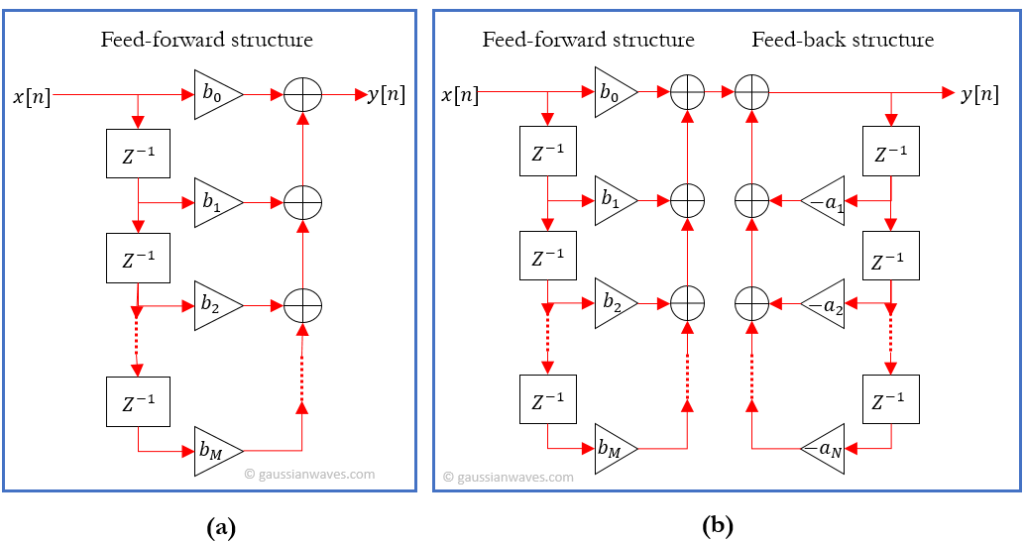
\includegraphics[width=1.0\columnwidth]{images/fir_vs_iir_diagram.png}
	\end{center}
	\caption{A diagram displaying the difference between Finite impulse response filters, only using previous input, and Infinite impulse response filters, using previous inputs and previous outputs resulting in a feedback loop \cite{fir_vs_iir_diagram}}
	\label{fig:fir_vs_iir_diagram}
\end{figure}


\section{Pre-whitening}
Back in 1948 a mathematician, electrical engineer, and cryptographer named C.E. Shannon published a pioneering paper that formed the basis of information theory \cite{shannon}. In this paper it is shown that repetition does not carry information, and that the maximum information transfer occurs when a signal is truly random. Imagine a signal with only a single frequency component. After measuring a few samples of the signal the conlusion is drawn that this is a 50Hz signal. Since it is possible to predict the value of every future measurement of the signal after drawing this conclusion it becomes unnecessary to continue measuring the signal because it will not give any new information. A repeating pattern is predictable, and predictable events carry no information.

The polar opposite of a signal containing a single frequency that is therefore predictable and carries little information is a signal that contains all frequencies an equal amount. This is called a white noise signal and carries the maximum amount of information because there exists no repetition and therefore every sample carries new, unpredictable information.

Between the existance of a signal containing a single frequency, and a signal containing all frequencys (white noise), all other signals exist and have certain frequencies that are more 'present' than other frequencies. These signals have different degrees of predictability (and thus information density), and the degree of predictability is determined by how closely the frequency content resembles white noise.

Whitening is a filtering technique that tries to equalize the presence of frequency components in a signal to approximate white noise and thus increase information density. It reduces the random error and yields a larger dynamic range because the small frequency components that contribute to the 'randomness' of the signal but not so much to the value of the measurement sample become more present \cite{time_series_analysis_methods} (Chapter: 5.4.9. Zero-Padding and Prewhitening). The serial correlation of the signal is decreased by reducing the presence of 'predictable' signals, which increases the randomness and thus information density \cite{serial_correlation_definition}. 

This previous information manifests itself in sEMG signal processing by the fact that the measured sEMG signal is not white. Some frequency components are much more present than others, but all frequencies equally contribute to the indication of muscle contraction. To get a more accurate indication of muscle contraction the signal should be whitened to increase the information of each sample.

Whitening in real-time is achieved through a digital filter with a frequency response that when multiplied with the sEMG signal frequency spectrum yields a white noise spectrum.

To summarize: Whitening reduces the power of repeating frequencies and increase the power of random frequencies in the signal. An example is given in figure \ref{fig:whitening_example}.

\begin{figure}[h!t]
	\begin{center}
		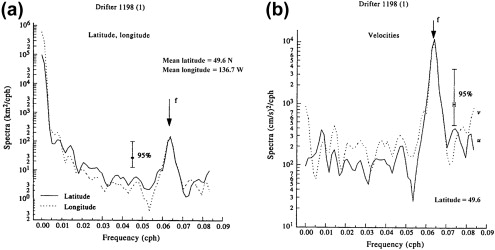
\includegraphics[width=0.7\columnwidth]{images/prewhitening_example.jpg}
	\end{center}
	\caption{An example of whitening a signal. The indicated peak contains the 'random' signal of interest. By whitening the powerful lower frequencies it is possible to give the information-carrying peak more presence on the signal \cite{time_series_analysis_methods}}
	\label{fig:whitening_example}
\end{figure}


\section{Envelope detection}

\begin{figure}[h!t]
	\begin{center}
		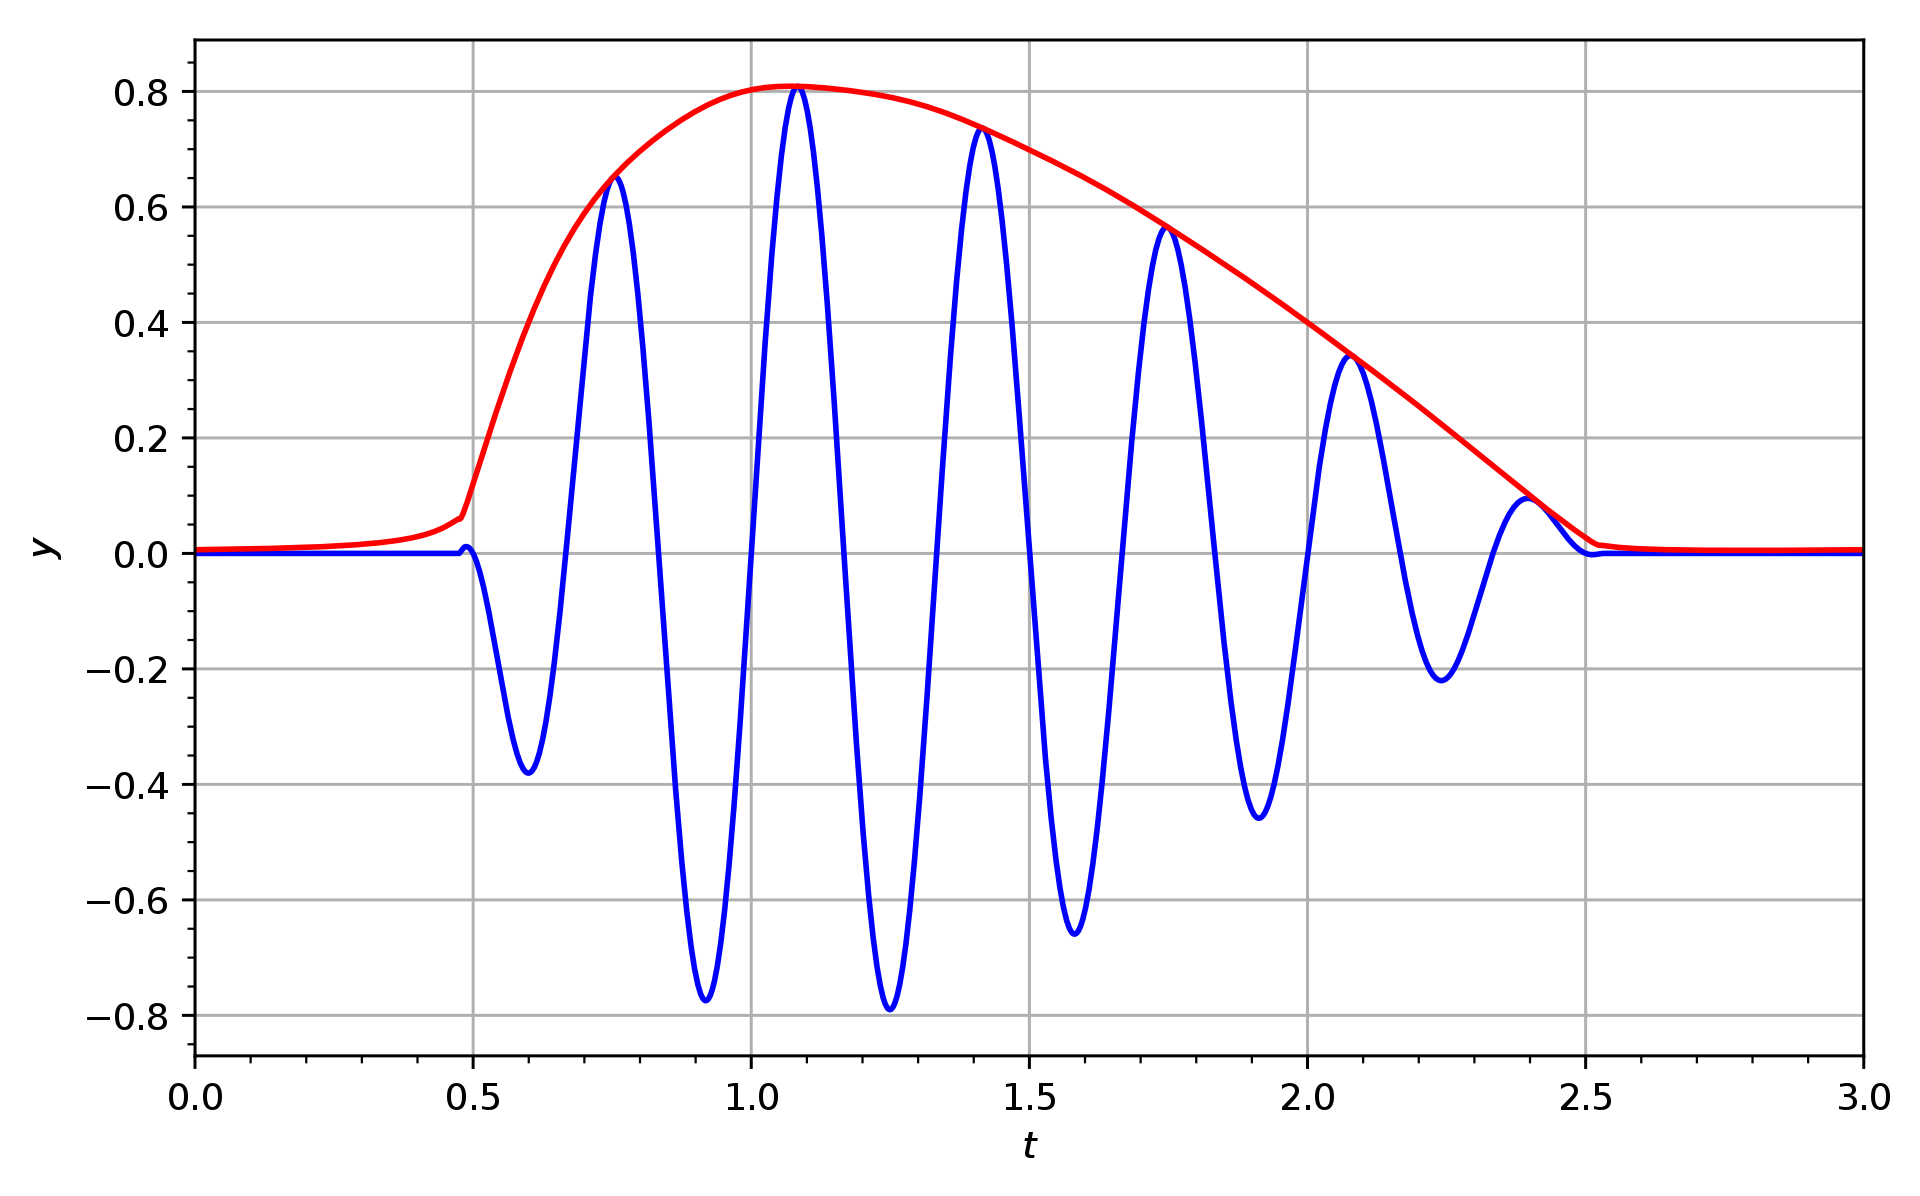
\includegraphics[width=0.7\columnwidth]{images/envelope_wikipedia.png}
	\end{center}
	\caption{Illustrating envelope detection of an analytical signal \cite{envelope_wikipedia}}
	\label{fig:envelope_wikipedia}
\end{figure}

\begin{figure}[h!t]
	\begin{center}
		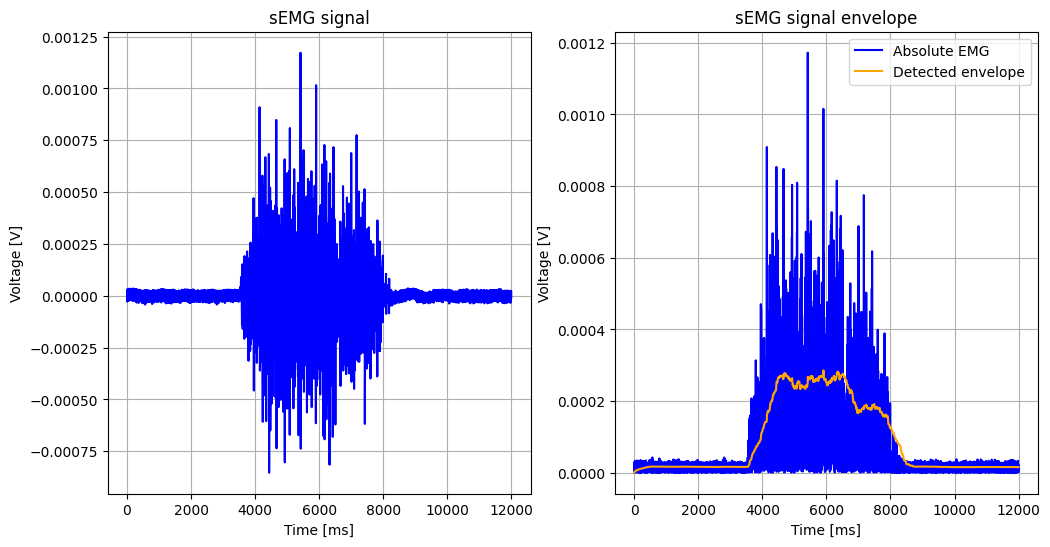
\includegraphics[width=1.0\columnwidth]{images/amplitude_force_estimation_example.png}
	\end{center}
	\caption{On the left a time-domain sEMG signal. On the right an example of force estimation is presented. By taking the absolute value of the sEMG signal on the left, calculating the envelope, and recognizing that the force is a linearly scaled version of the envelope it is possible to estimate the force from the sEMG signal.}
	\label{fig:amplitude_estimation_example}
\end{figure}

As mentioned earlier the amplitude of a measured sEMG signal scales approximately linear with how much a skeletal muscle is contracted \cite{adaptive_filter_dry_electrode}. Since the raw EMG signal consists of stochastic and unpredictable noise it is difficult to draw conclusions about the degree of muscle contraction when solely looking at individual samples \cite{semg_signals_analysis_and_applications}. By drawing an outline of the peaks of the signal a much more informative picture can be drawn. This is called an envelope and an illustration of this process can be found in figure \ref{fig:envelope_wikipedia}. In the case of more random sEMG signals it is preferred to perform full wave rectification on the signal before calculating the envelope so that all of the signal energy is taken into account \cite{semg_signals_analysis_and_applications}. Applying this concept to an sEMG signal can be found in figure \ref{fig:amplitude_estimation_example}.

Computationally envelope detection can be achieved in a number of different methods where "speed", or how much the detected envelope lags behind the true signal envelope, is traded against accuracy or noisiness \cite{dsp_good_bad_ugly}. A few different envelope detection techniques are discussed in \cite{rose2011electromyogram}.

\subsection{Moving average}
A moving average filter is a special type of FIR filter with coefficients that are all have the value of $\frac{1}{n}$ where $n$ is the number of samples over which the average is taken. Thus the value of every smoothened sample is calculated to be the average of the previous $n$ samples. The upside of a moving average filter is that is is very simple to implement and introduces zero phase shift. A downside of a moving average filter is that it lags behind the signal by its very definition: a change in a static signal level is only properly reflected after $n$ samples. The sEMG signal must also be rectified before this method can be applied because EMG signal has approximately zero mean due to its oscillatory behaviour \cite{rose2011electromyogram}. 

\subsection{IIR Lowpass filter}
A lowpass filter such as a Butterworth or Chebyshev can be used to determine the envelope of a rectified signal in a more 'responsive' (less lag) method compared to a moving average filter. The downside of this filter is that it introduces phase shift unless applied in forward and backward direction \cite{rose2011electromyogram} which is not possible in real-time signals without introducing a static delay of a number of samples that equals the number of filter coefficients.

\subsection{Root Mean Square}
The Root Mean Square (RMS) of a signal is the square root of average power of a signal for a given period of time, a definition is given in equation \ref{eq:rms}. A useful property of RMS is that when it is applied to a signal with Gaussian distribution the RMS amplitude of the source is the same as the standard deviation of the distribution \cite{rms_standard_deviation}. In other words this means that RMS can extract the signal power of all frequencies in a signal in the time-domain if the frequencies are normally distributed.Since the probability density of surface EMG is approximately Gaussian, RMS should theoretically be the maximum likelihood estimator of EMG amplitude \cite{semg_signals_analysis_and_applications}.

\begin{equation}
    RMS = \sqrt{\frac{1}{n} (x[1]^2 + x[2]^2 + \cdots + x[n]^2)}
    \label{eq:rms}
\end{equation}

\section{Standard sEMG signal processing}\label{section:standard_semg_processing}
A conventional static real-time sEMG signal processing chain is described in \cite{muscle_force_estimation}. The relevant steps are as follows:
\begin{itemize}
    \item Highpass filter to remove DC
    \item Bandpass filter 20-300 hz
    \item Notch filter at 50hz
    \item Half-wave rectification
    \item Lowpass filter for envelope detection
\end{itemize}

This signal processing chain will also be tested in this report and compared to alternative techniques.